\section{UHC Backend}

% two steps, first without mod
\begin{frame}[fragile]{UHC Compiler}
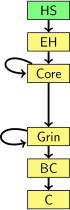
\includegraphics{uhc-arch-extr.png}
\end{frame}

\begin{frame}[fragile]{UHC Compiler}
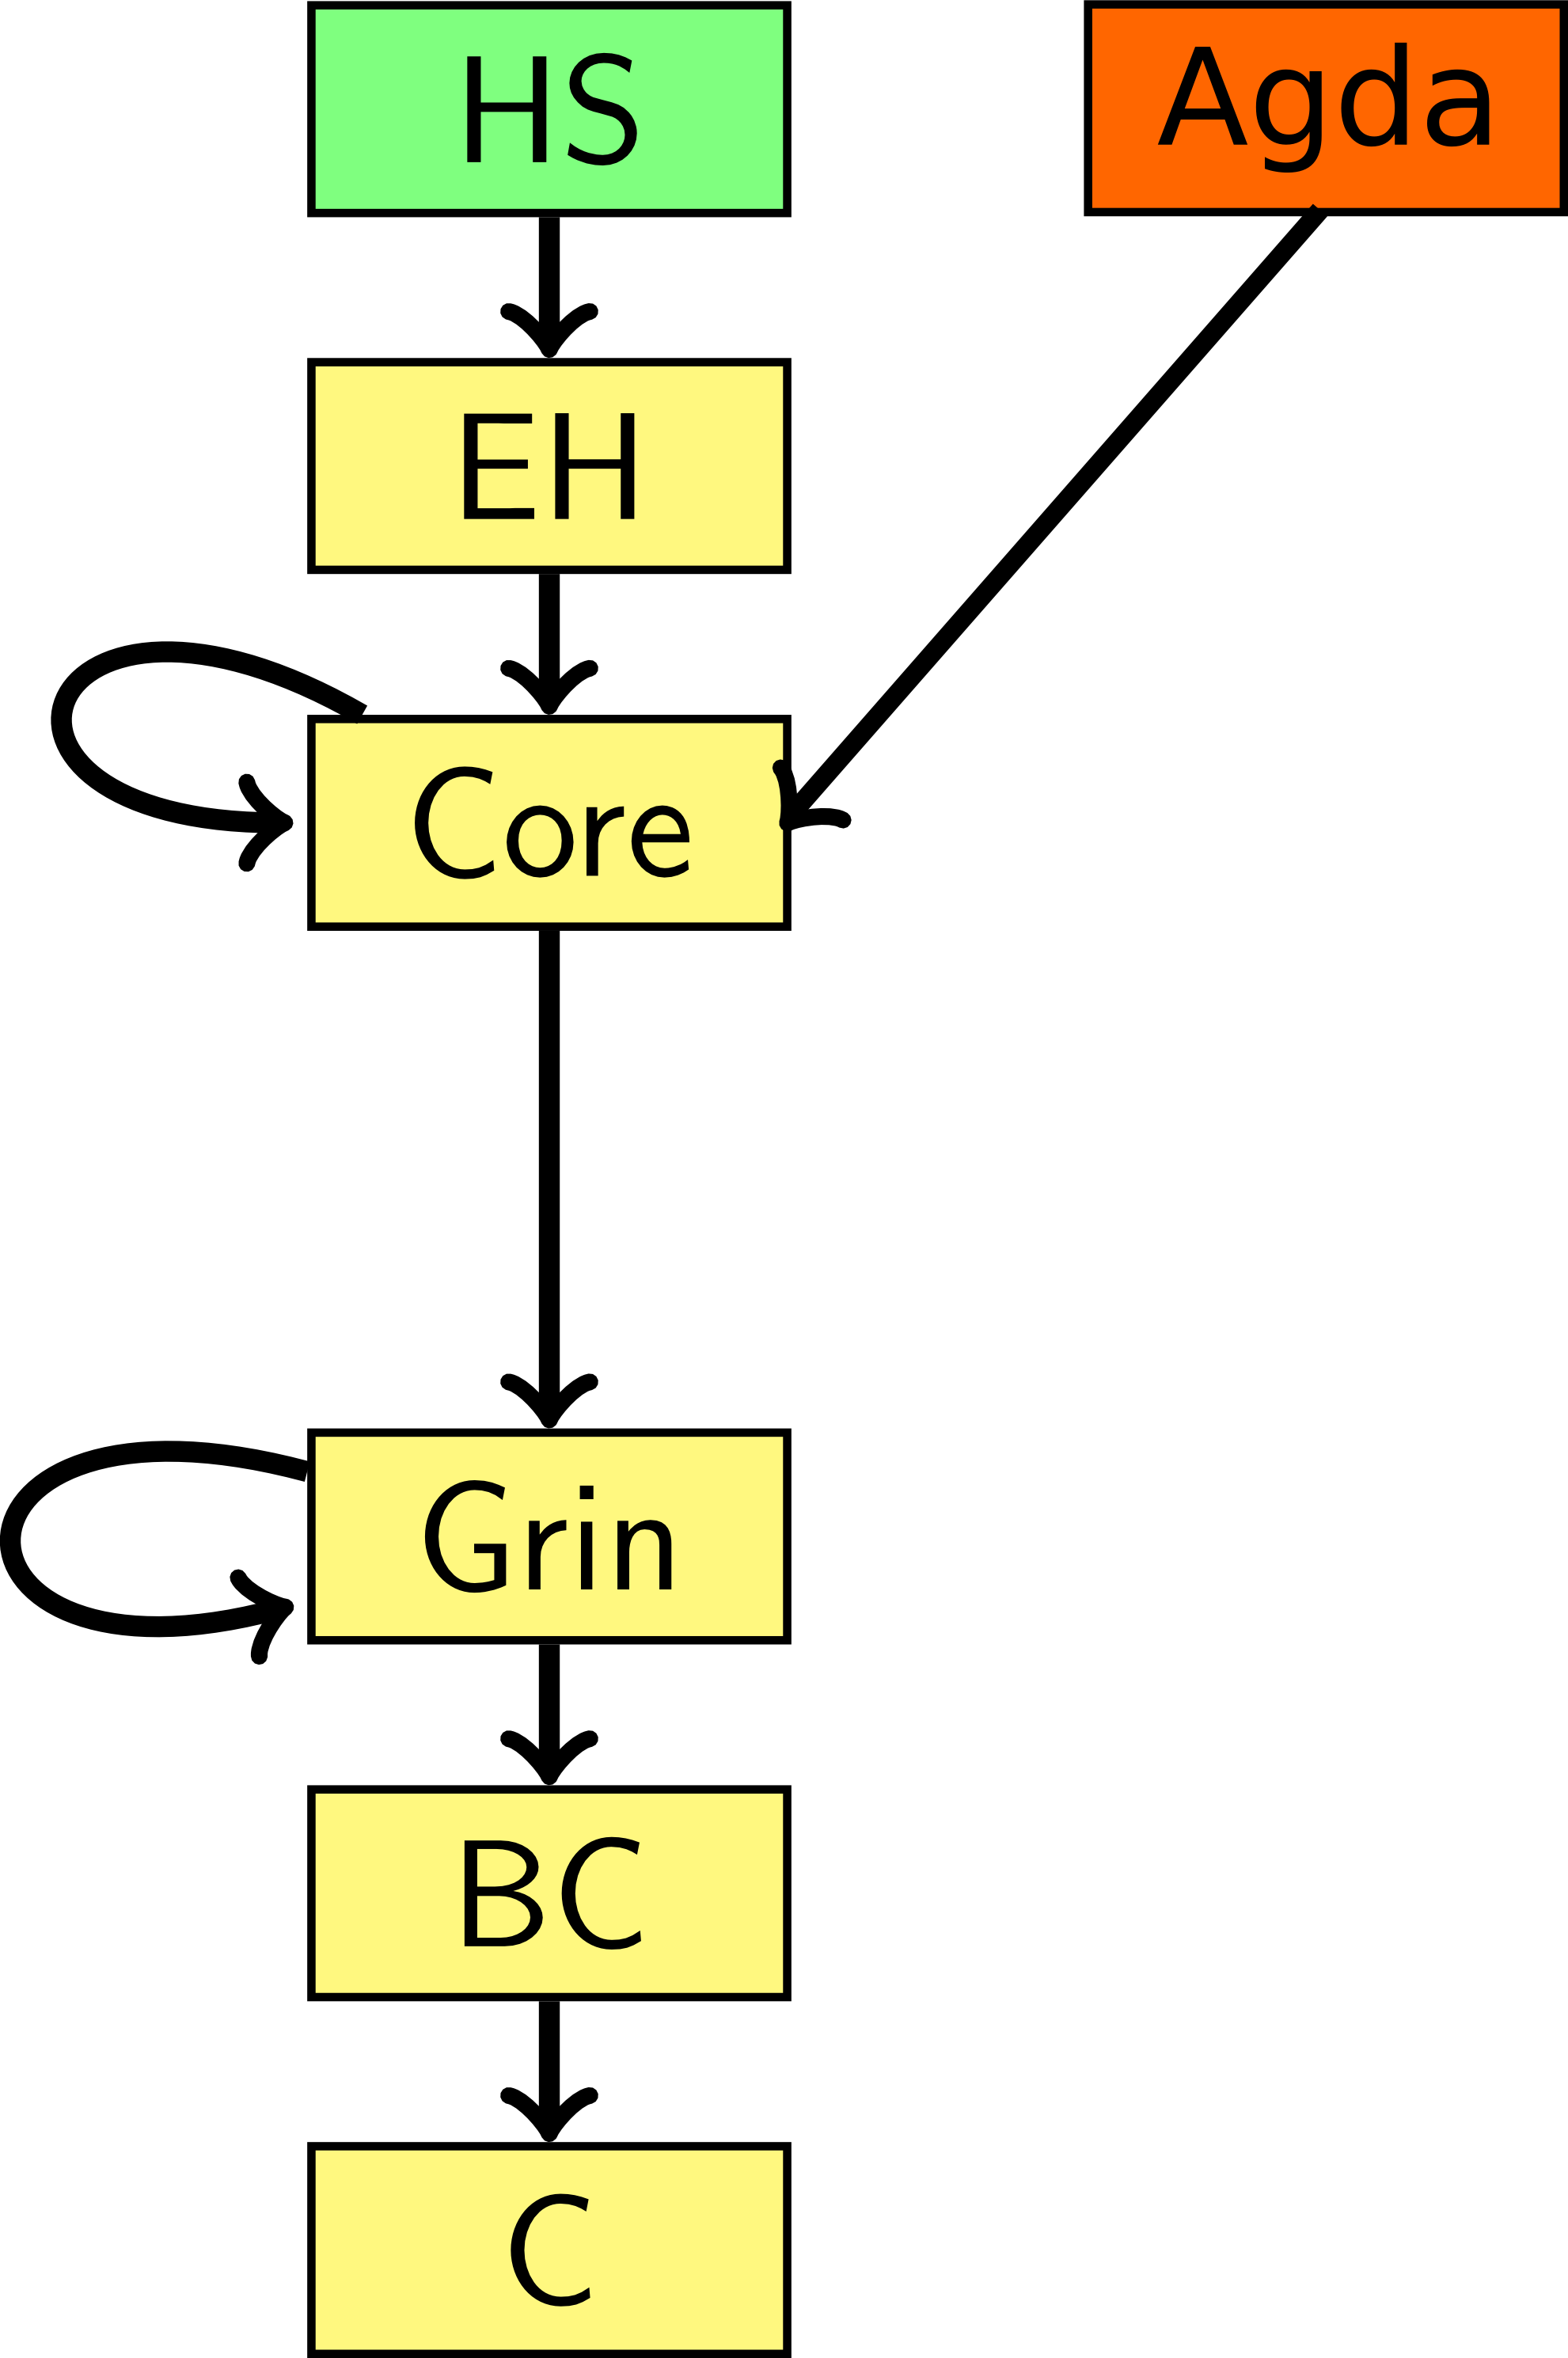
\includegraphics{uhc-arch-extr-mod.png}
\end{frame}


\begin{frame}[fragile]{UHC Backend}
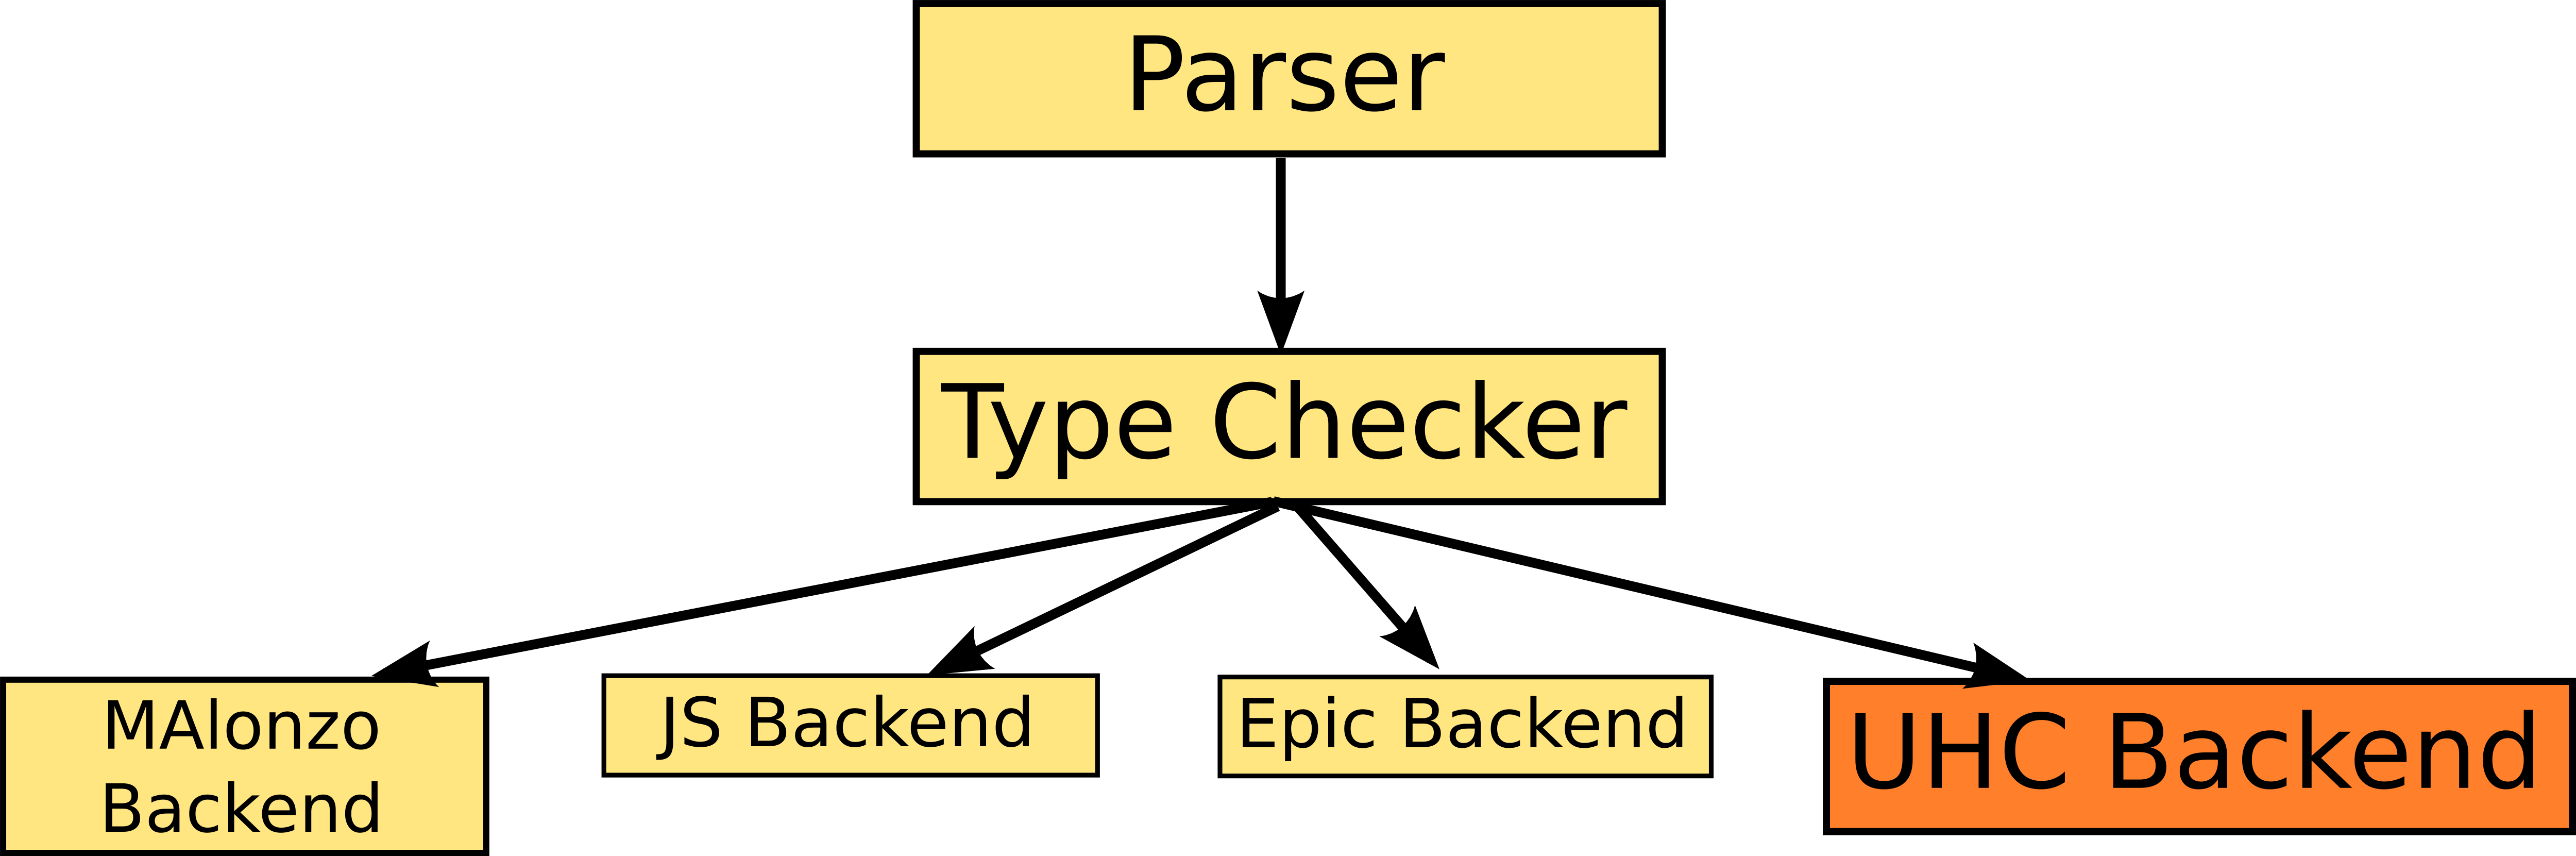
\includegraphics[width=250px]{agda-arch-with-uhc.png}
\end{frame}


\begin{frame}{Epic vs UHC Core}
\begin{tabular}{c r l c r l}
\hline
\multicolumn{3}{l}{Epic Language} & \multicolumn{3}{l}{UHC Core} \\
\hline
$t$ & $::=$ & $x$               & $t$ & $::=$ & $x$ \\
& \textbar & $t$ $\vec{t}$            & & \textbar & $t$ $t$ \\
& \textbar & $\lambda x \rightarrow t$ & & \textbar & $\lambda x \rightarrow t$ \\
& \textbar & Con $i$ $\vec{t}$        & & \textbar & Con $i$ $\vec{t}$ \\
& \textbar & if $t$ then $t$ else $t$ & & & \\
& \textbar & case $t$ of $\vec{alt}$  & & \textbar & case $t$ of $\vec{alt}$ \\
& \textbar & let $x$ = $t$ in $t$     & & \textbar & let $x$ = $t$ in $t$ \\
& &                                   & & \textbar & let! $x$ = $t$ in $t$ \\
& \textbar & lazy $t$                 & & & \\
%& \textbar & $t$ $!$ $i$              & & & \\
& \textbar & $i$                      & & \textbar & $i$
%\\
%$alt$ & ::= & Con $i$ $\vec{x}$ $\rightarrow$ $t$     & $alt$ & $::=$ & Con $i$ $\vec{x}$ $\rightarrow$ $t$ \\
%& \textbar & $i$ $\rightarrow$ $t$                    & & & \\
%& \textbar & default $\rightarrow$ $t$                & & \textbar & default $\rightarrow$ $t$
\end{tabular}
\end{frame}

\begin{frame}[fragile]{UHC Backend}
\begin{itemize}
\item UHC Core was not intended as public API
\item Undocumented assumptions inside UHC
\pause
\begin{lstlisting}[language=Haskell]
case x of
  []     -> a
  (x:xs) -> b
\end{lstlisting}
is not the same as
\begin{lstlisting}[language=Haskell]
case x of
  (x:xs) -> b
  []     -> a
\end{lstlisting}
%\begin{itemize}
%    \item E.g. alt
%\end{itemize}
\end{itemize}
\end{frame}

\begin{frame}{UHC Backend - What works?}
\begin{itemize}
\item (Dependent) dataypes, functions
\item Compiling single Agda modules
\item Agda - Haskell FFI, but involves manual work
\end{itemize}
\end{frame}

\begin{frame}
Demonstration
\end{frame}

\begin{frame}{UHC Backend - Future work}
\begin{itemize}
\item Support whole Agda language
  \begin{itemize}
  \item Multiple modules
  \item Complete IO bindings
  \item Agda Standard Library
  \end{itemize}
\item Optimizations
\item Improve Agda - Haskell FFI
\item Agda support for Cabal
\item Contracts for FFI
\end{itemize}
\end{frame}
